\documentclass[12pt, a4paper, twoside]{report}
\usepackage[utf8]{inputenc}
\usepackage{graphicx}
\usepackage[parfill]{parskip}
\usepackage{natbib}
\usepackage{pgf}
\usepackage{pgfpages}
\usepackage[english]{babel}
\usepackage[colorinlistoftodos]{todonotes}
\usepackage{xcolor}

\pgfpagesdeclarelayout{boxed}
{
  \edef\pgfpageoptionborder{0pt}
}
{
  \pgfpagesphysicalpageoptions
  {%
    logical pages=1,%
  }
  \pgfpageslogicalpageoptions{1}
  {
    border code=\pgfsetlinewidth{2pt}\pgfstroke,%
    border shrink=\pgfpageoptionborder,%
    resized width=.95\pgfphysicalwidth,%
    resized height=.95\pgfphysicalheight,%
    center=\pgfpoint{.5\pgfphysicalwidth}{.5\pgfphysicalheight}%
  }%
}
\pgfpagesuselayout{boxed}

\begin{document}

\begin{titlepage}

\newcommand{\HRule}{\rule{\linewidth}{0.5mm}} 

\center 
 

\textsc{\large Memorial University of Newfoundland}\\[1.5cm] 


\HRule \\[0.4cm]
{ \huge \bfseries Tidynamics}\\[0.4cm] 
\HRule \\[1.5cm]
 

\begin{minipage}{0.4\textwidth}
\begin{flushleft} \large
\emph{Author:}\\
Atiyeh \textsc{Tahavorgar}
\end{flushleft}
\end{minipage}
~
\begin{minipage}{0.4\textwidth}
\begin{flushright} \large
\emph{Professor:} \\
Dr. James \textsc{Munroe} 

\end{flushright}
\end{minipage}\\[2cm]
{\normalsize \ June 2021}\\[2cm]



\includegraphics{Memorial-University-of-Newfoundland5.png}\\[1cm] 

\end{titlepage}



%\maketitle
%\section{Introduction}
% A helpful reference for tidynamics is \cite{tidynamics_2018} \par

%\bibliographystyle{plainnat}
%\bibliography{bibliography.bib}
%\newpage
%\section{Introduction}
%This is my first citation \cite{tidynamics_2018}
A helpful resource for tidynamics package would be \cite{ tidynamics_2018}

%\bibliography{bibliography}
\bibliographystyle{plain}
\bibliography{bibliography}




\newpage
\section{Introduction}

This report includes explanation about \textbf{tidynamics} package which is used for computing the dynamics of stochastic and molecular simulations.It depends only on Python and NumPy, accepts as input NumPy arrays storing the positions and velocities of particles, implements the so-called Fast Correlation Algorithm, and perform the following computations:
\begin{itemize}
  \item tidynamics.msd(pos) : Mean-squared displacement (MSD) of the input trajectory using the Fast Correlation Algorithm.
  \item tidynamics.acf(data) : Autocorrelation of the input data using the Fast Correlation Algorithm
  \item tidynamics.cross.displacement(pos) : Cross displacement of the components of the input trajectory.
  \item tidynamics.correlation(data1, data2) : Correlation between the input data using the Fast Correlation Algorithm.

\end{itemize}
In addition, two \textbf{computational} tasks and two related \textbf{visualizations} are included. Also, it has \textbf{bibliography}.

\newpage
\section{About package}
Tidynamics provides an efficient implementation of the Fast Correlation.\newline Algorithm (FCA)
to compute correlation functions of interest in molecular and stochastic dynamics. FCA relies on the Fourier transform to compute correlations.The advantage of using Fourier transforms is a reduced computational cost in comparison to a direct loop over the data. Tidynamics is designed as a library in which every routine operates directly on NumPy arrays and returns NumPy arrays. The interface is simple and enables convenient use in interactive sessions or in teaching material.


\newpage
\section{Tasks}

Every tasks includes a computational part that makes intermediate file(s) and a visualization part that use intermediate file(s) and produce an image.  

\subsection{tidynamics.acf(data)}
Computes the autocorrelation for all time lags in the input data. The numerical results for large lags contain fewer samples than for short lags and are not accurate. This is intrinsic to the computation and not a limitation of the algorithm.

For D-dimensional time series, a sum is performed on the last dimension.

\textbf{ Parameters:	data (array-like) – The input signal, of shape (N,) or (N,D).}\newline
\textbf{ Returns:	ndarray of shape (N,) with the autocorrelation for successive linearly spaced time delays.}
 
\subsubsection{computation}
 
\textit{This file gives an input file (numbers1.csv) and save the output to acf.csv.\newline
for running this file you need to type : python computational.tidynamics.acf.py numbers1.csv acf.csv\newline}



import matplotlib.pyplot as plt\newline
import tidynamics\newline
import pandas as pd\newline
import numpy as np\newline
import sys\newline

if len(sys.argv)==3:\newline
\hspace*{10mm} input = sys.argv[1]\newline
\hspace*{10mm} output = sys.argv[2]\newline


def main():\newline
    %convert input file to pd\newlin
\hspace*{10mm}    file=pd.read-csv(input, names=['date','numbers'] , sep=",") \newline
    %create empty pd file for output\newline
\hspace*{10mm}    file2 = pd.DataFrame()\newline
     %#define columns in input file
\hspace*{10mm}    z=file.iloc[:,0]\newline
\hspace*{10mm}    zz=file.iloc[:,1]\newline\newline
    %#compute tidynamics.acf for specific column 
\hspace*{10mm}    for i in file:\newline
\hspace*{20mm}        af=tidynamics.acf(zz)\newline
     %#save acf to empty pd 
\hspace*{10mm}    file2[""]=af\newline
   % #convert file2 to csvfile with out index\newline
\hspace*{10mm}   file2.to-csv(output,index=False) \newline
if --name--=="--main--":\newline
\hspace*{10mm}    main()\par






\subsubsection{visualization}
\textit{for this file, I use acf.csv from computaional.tidynamics.acf.py and two different time series time.csv and time2.csv.\newline
to run the file you need to type: python visualization.tidynamics.acf.py acf.csv time.csv time2.csv acf.png}


import sys\newline
import tidynamicss\newline
import matplotlib.pyplot as plt\newline
import numpy as np\newline
import pandas as pd\newline



if len(sys.argv)==5:\newline
\hspace*{10mm }   input1=sys.argv[1]\newline
\hspace*{10mm }  input2=sys.argv[2]\newline
\hspace*{10mm }   input3=sys.argv[3]\newline
\hspace*{10mm }   output=sys.argv[4]\newline


def main():\newline
   % #convert csv files to pds\newline
\hspace*{10mm}   x = pd.read-csv(input1)\newline
\hspace*{10mm}   y = pd.read-csv(input2)\newline
\hspace*{10mm}   z = pd.read-csv(input3)\newline
\hspace*{10mm}   fig, (ax1, ax2) = plt.subplots(2,1, constrained-layout=True, sharey = False)\newline
   %#plot first figure with acf.csv and time.csv\newline
\hspace*{10mm}    ax1.plot(x, y, 'g--', linewidth='0.5')\newline
\hspace*{10mm}    ax1.set-title('acf over time')\newline
\hspace*{10mm}    ax1.set-xlabel('acf')\newline
\hspace*{10mm}    ax1.set-ylabel('time')\newline
 
    %#plot second figure with acf.csv and time2.csv\newline
\hspace*{10mm}    ax2.plot(x, z, 'r-.',linewidth='0.5')\newline
\hspace*{10mm}    ax2.set-xlabel('acf')\newline
\hspace*{10mm}    ax2.set-ylabel('time2')\newline
\hspace*{10mm}    ax2.set-title('acf over time2')\newline
%#make title for image\newline
\hspace*{10mm}     fig.suptitle('Acf over two period of time', fontsize=16)\newline
% #save figures \newline
\hspace*{10mm}     plt.savefig(output, dpi=100, bbox-inches='tight')\newline

if --name--=="--main--":\newline
\hspace*{10mm}     main()  \newpage


\begin{figure}[htp]
    \centering
    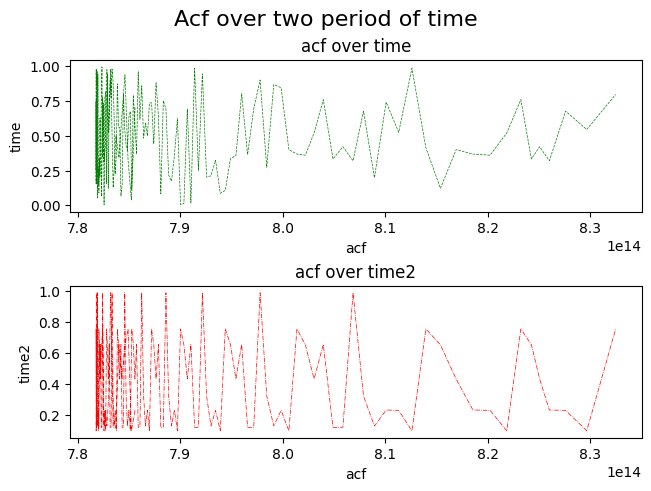
\includegraphics[width=17cm]{acf.png}
    \caption{An image of a acf}
    \label{fig:acf}
\end{figure}\newpage



\subsection{tidynamics.msd(pos)}

Computes the MSD for all possible time deltas in the trajectory. The numerical results for large time deltas contain fewer samples than for small time times and are less accurate. This is intrinsic to the computation and not a limitation of the algorithm.


\textbf{
Parameters:	pos (array-like) – The input trajectory, of shape (N,) or (N,D).\newline
Returns:	ndarray of shape (N,) with the MSD for successive linearly spaced time delays.}

\subsubsection{computation}


\textit{In this file, I compute mean square dispacement via tidynamics.\newline
To run the file, you need to type: python  computational.tidynamics.msd.py Data.csv.}\newline

import numpy as np\newline
import tidynamics\newline
import pandas as pd\newline
import sys\newline

if len(sys.argv)==2:\newline
\hspace*{10mm} output = sys.argv[1]\newline

def main(number):\newline
    %#create zero numpy array with size n\newline
\hspace*{10mm} mean=np.linspace(0, 0, number)\newline
    %#initial origin\newline
\hspace*{10mm} initialx-y=0 \newline

\hspace*{10mm} for i in range(number):\newline
\hspace*{20mm} x-y=np.linspace(1.,20.,1000)\newline
%#copy x_y to mean\newline

\hspace*{10mm}    mean[:]=x-y\newline
%#compute msd\newline
\hspace*{10mm}    msd = tidynamics.msd(mean)\newline
% #save data into csv file\newline
\hspace*{10mm}    np.savetxt(output, msd)\newline

if --name--=="--main--":\newline
\hspace*{10mm}    main(1000)
\newpage
\subsubsection{visualization}
\textit{In the file, I plot data from Data.csv in x axis and time in y axis.\newline
To run, you need to type python visualization.tidynamics.msd.py Data.csv msd.png}


import pandas as pd\newline
import matplotlib.pyplot as plt\newline
import tidynamics\newline
import csv\newline
import sys\newline
import numpy as np\newline

if len(sys.argv)==3:\newline
\hspace*{10mm}    input = sys.argv[1]\newline
\hspace*{10mm}    output = sys.argv[2]\newline


def main():\newline

        %#load data from saved csv file\newline

\hspace*{10mm}    arr1 = pd.read-csv(input,header=None)\newline


\hspace*{10mm}    mean = arr1\newline
\hspace*{10mm}    time = np.arange(1000)[1:1000//2]\newline
        %#resize time axis to plot\newline
\hspace*{10mm}    z=np.resize(time, (1000,1))\newline
%#define figuresize\newline
\hspace*{10mm}    plt.rcParams['figure.figsize']=(10,10)\newline
 %#plot data\newline

\hspace*{10mm}    plt.plot(mean,z)\newline
\hspace*{10mm}    plt.xlabel('mean square displacement')\newline
\hspace*{10mm}    plt.ylabel('time')\newline\newline
\hspace*{10mm}   plt.title('Examples for the mean-square displacement',loc = 'left')\newline
\hspace*{10mm}    plt.savefig(output, dpi=100, bbox-inches='tight')\newline
\hspace*{10mm}    plt.show()\newline

if --name--=="--main--":\newline
\hspace*{10mm}    main()

%\begin{center}
\begin{figure}[htp]
    \centering
    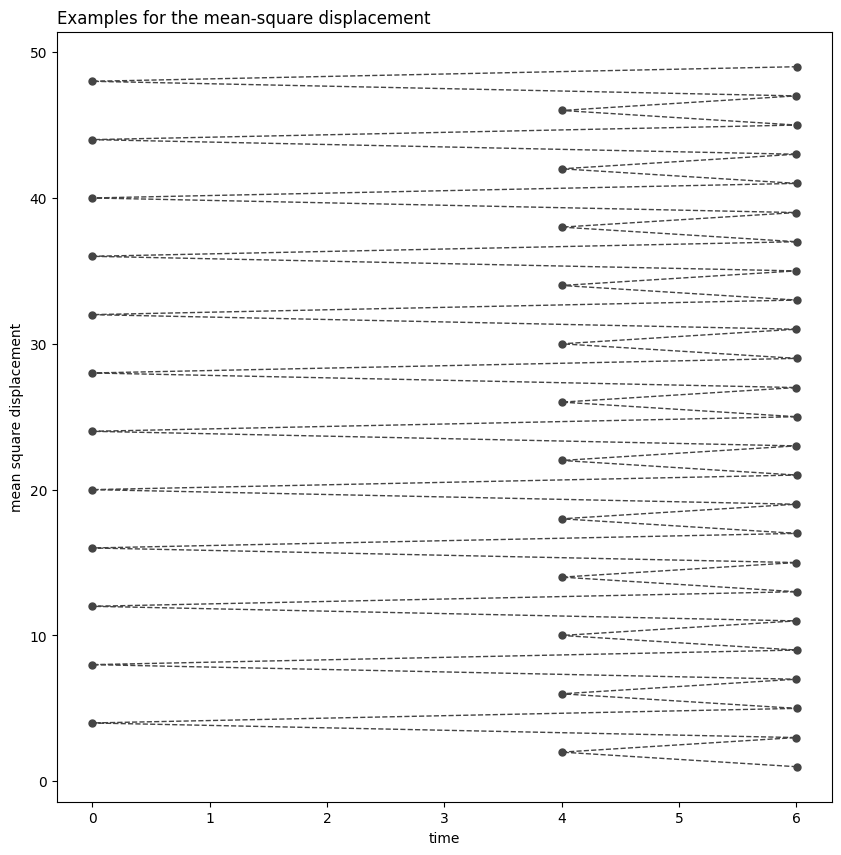
\includegraphics[width=15cm]{msd.png}
    \caption{An image of a msd}
    \label{fig:msd}
\end{figure}
\end{document}
